\section{Résultats}

\begin{minipage}{\textwidth}
    \begin{wrapfigure}{R}{0.55\textwidth}
        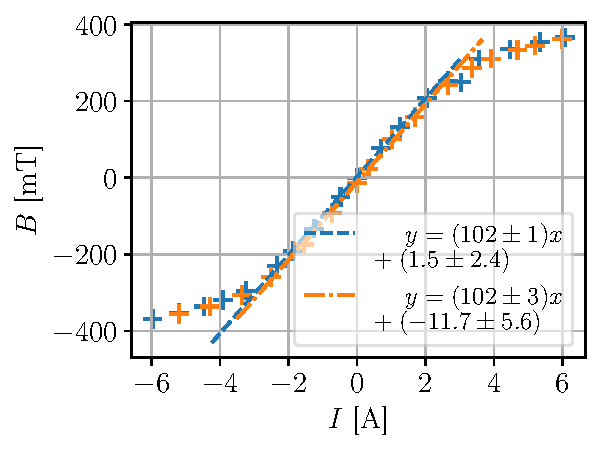
\includegraphics[width=\linewidth]{figures/calibration.pdf}
        \caption{Variation de l'amplitude du champ magnétique en fonction du courant sur un cycle \(I_\textrm{max} \rightarrow 0 \rightarrow -I_\textrm{max} \rightarrow 0 \rightarrow I_\textrm{max}\).}
        \label{fig:callibration}
    \end{wrapfigure}

    \paragraph*{Étalonnage du champ d'induction}
    La \autoref{fig:callibration} montre comment varie le champ magnétique en fonction du courant. Ici, \(I_\textrm{max} = 6\) \si{\ampere}. Par souci de clarté, les erreurs sur les mesures ne sont pas affichées dans cette figure et sont de l'ordre de 2\%, dont les calculs sont détaillés dans \autoref{sec:erreurs}. Les points bleus correspondent à la partie descendante du cycle et les points oranges à la partie montante. Deux fit linéaire on été réalisés sur la partie linéaire (entre -3 \si{\ampere} et 3 \si{\ampere}), 1 pour chaque sens, et mettent en évidence une légère hystérèse, puisque les deux droites sont décalées, d'ordonnée à l'origine \(\beta_1 = (1.5 \pm 2.4)\) pour la partie \(I_\textrm{max} \rightarrow 0 \rightarrow -I_\textrm{max}\) contre \(\beta_2 = (-11.7 \pm 5.6)\) pour la partie \(-I_\textrm{max} \rightarrow 0 \rightarrow I_\textrm{max}\).

    \paragraph*{Tensions résiduelles}
    Le \autoref{tab:tension_residuelle} montre les tensions résiduelle dans deux échantillons d'InP dopés au Si d'épaisseurs 1 \si{\micro\meter} et 2 \si{\micro\meter}. Les mesures ont été réalisées avec un champ magnétique de 0 \si{\milli\tesla} et un courant \(I = 1.002 \pm 0.001\) pour le premier échantillon \(I = (1.001 \pm 0.001)\) \si{\milli\ampere} pour le deuxième échantillon.
\end{minipage}

\begin{table}[h]
    \centering
    \begin{tabulary}{\textwidth}{C C C C}
        \toprule
        Configuration \si{\micro\meter} & Tension (\(a = 1\) \si{\micro\meter}) [\si{\milli\volt}] & Tension (\(a = 2\) \si{\micro\meter}) [\si{\milli\volt}] \\
        \midrule
        \(I_{13}U_{24}\) & \(68.74 \pm 0.01\) & \(27.02 \pm 0.01\) \\
        \(I_{31}U_{42}\) & \(68.69 \pm 0.01\) & \(27.12 \pm 0.01\) \\
        \(I_{24}U_{13}\) & \(39.93 \pm 0.01\) & \(24.78 \pm 0.01\) \\
        \(I_{42}U_{31}\) & \(40.12 \pm 0.01\) & \(24.76 \pm 0.01\) \\
        \bottomrule
    \end{tabulary}
    \caption{Tension résiduelle pour différentes configuration et 2 épaisseurs de l'échantillon InP dopés au Si}
    \label{tab:tension_residuelle}
\end{table}

\paragraph*{Détermination de la constante de Hall}
Afin de déterminer la constante de Hall des deux échantillon d'InP dopés au Si, un champ magnétique constant de \(B = (348 \pm 7)\) \si{\milli\tesla} et \(B = 383 \pm 7\) \si{\milli\tesla} à été appliqués aux échantillons de 1 \si{\micro\meter} et 2 \si{\micro\meter} respectivement. La configuration \(I_{24}U_{13}\) a été choisie en raison de sa faible tension résiduelle. Les \autoref{fig:inpV(I)} et \autoref{fig:inpV(B)} montrent la variation de la tension de Hall en fonction du courant dans l'échantillon et du champ magnétique respectivement. Les coefficients des regressions linéaires permettent de déterminer à l'aide de l'\autoref{eq:R_H} les valeurs du coefficient de Hall \(R_H\) et avec l'\autoref{eq:N} la densité de porteurs de charge \(N\). Les résultats sont reportés dans le \autoref{tab:RH_N}.

\begin{table}[h]
    \centering
    \begin{tabulary}{\textwidth}{C C C C C}
        \toprule
        Échantillon & \(R_H^B\) [\si{\meter\cubed\per\coulomb}] & \(R_H^I\) [\si{\meter\cubed\per\coulomb}] & \(N^B\) [\si{\per\meter\cubed}] & \(N^I\) [\si{\per\meter\cubed}] \\
        \midrule
        1 \si{\micro\meter} & \((-2.40 \pm 0.05) \cdot 10^{-3}\) & \((-2.24 \pm 0.02) \cdot 10^{-3}\) & \((2.60 \pm 0.05) \cdot 10^{21}\) & \((2.79 \pm 0.03) \cdot 10^{21}\) \\
        2 \si{\micro\meter} & \((-1.47 \pm 0.03) \cdot 10^{-3}\) & \((-1.62 \pm 0.01) \cdot 10^{-3}\) & \((4.25 \pm 0.08) \cdot 10^{21}\) & \((3.84 \pm 0.02) \cdot 10^{21}\) \\
        \bottomrule
    \end{tabulary}
    \caption{Valeurs de la constante de Hall \(R_H\) et densité de porteurs de charges \(N\) pour les échantillons d'épaisseur différente}
    \label{tab:RH_N}
\end{table}

\begin{figure}[h]
    \centering
    \begin{subfigure}{0.45\textwidth}
        \centering
        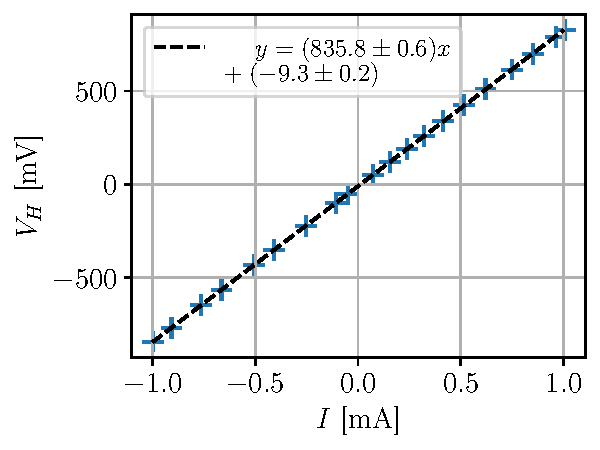
\includegraphics[width=\textwidth]{figures/U(I),InP1micro.pdf}
        \caption{}
    \end{subfigure}
    \begin{subfigure}{0.45\textwidth}
        \centering
        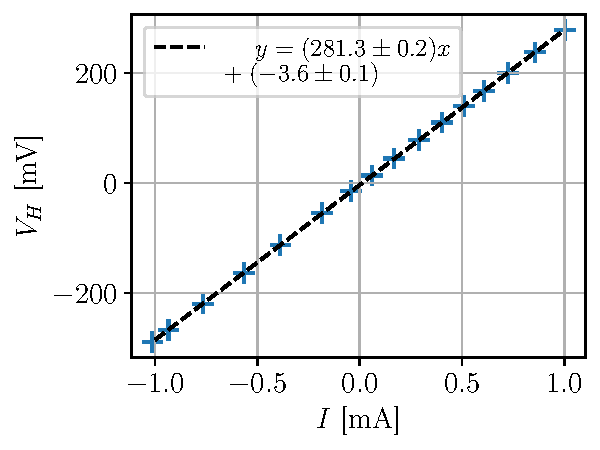
\includegraphics[width=\textwidth]{figures/U(I),InP2micro.pdf}
        \caption{}
    \end{subfigure}
    \caption{Tension en fonction de l'intensité pour l'échantillon InP d'épaisseur (a) 1 \si{\micro\meter} (b) 2 \si{\micro\meter}}
    \label{fig:inpV(I)}
\end{figure}

\begin{figure}[h]
    \centering
    \begin{subfigure}{0.45\textwidth}
        \centering
        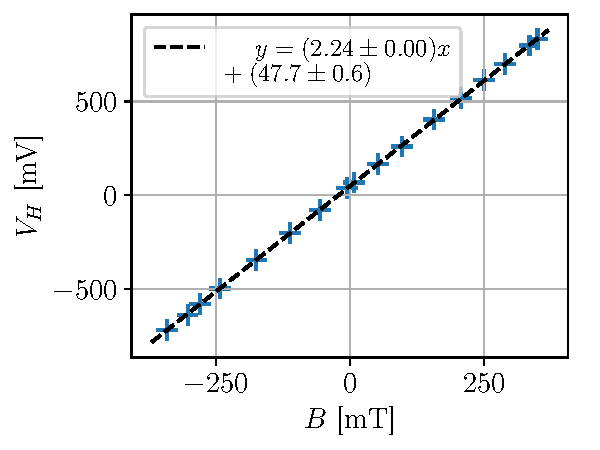
\includegraphics[width=\textwidth]{figures/U(B),InP1micro.pdf}
        \caption{}
    \end{subfigure}
    \begin{subfigure}{0.45\textwidth}
        \centering
        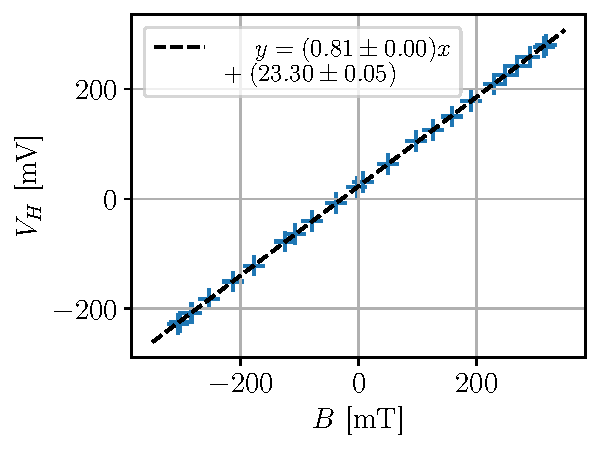
\includegraphics[width=\textwidth]{figures/U(B),InP2micro.pdf}
        \caption{}
    \end{subfigure}
    \caption{Tension en fonction de la norme signée du champ magnétique pour l'échantillon InP d'épaisseur (a) 1 \si{\micro\meter} (b) 2 \si{\micro\meter}}
    \label{fig:inpV(B)}
\end{figure}
